\section{Ecosystem Simulator}

Once the user selects the union of all species that must appear in all clusters of the terrain, it is necessary to determine a valid vegetation distribution for each cluster. To do so, an ecosystem simulator is used similarly to that in the work by Deussen et al \cite{Deussen1998} and Lane and Przemyslaw \cite{Lane2002}. Unlike these other ecosystem simulators, however, it isn't based on L-Systems and models both resource requirements and resource availability in greater detail. The purpose of ecosystem simulator is to determine, given a vegetative state, \textit{S$_{t}$} at time \textit{t}, the vegetative state \textit{S$_{t+n}$} at time \textit{t+n}, for any value of n.  \\

To do so, the simulation advances through time in monthly intervals and the strength of all plant instances are re-calculated at each iteration. Their strength depend not only on resource properties of the given month but also surrounding plants as they battle for these resources. Determining the set S = {P$_{1}$, P$_{2}$, P$_{3}$, ...} of plants which compete for resources with plant \textit{P$_{n}$} depends on the spatial reach of \textit{P$_{n}$}. Spatial awareness is therefore a key requirement of the simulation which is achieved by splitting the simulation area into a grid of cells as described in \textit{Gridded Simulation Area}.

Within each cell of the gridded simulation area, resources must be distributed to the different plant instances present. How this is done is described in \textit{Resource Distribution}. \\

Given the resources allocated to each plant instance, it is possible to calculate their strength. This is used as a representation of the plant's health and, consequentially, it's ability to survive and grow. Details about the plant's strength calculation and it's usage is discussed in \textit{Plant Strength} and \textit{Plant Strength Usage} respectively

\subsection{Gridded Simulation Area}

The simulation window used is one hundred by one hundred meters, accurate to the nearest centimetre. To easily model plant's interacting and battling for resources, the simulation window is split into cells to form a grid as illustrated in figure \ref{fig:simulation_grid}. 

\begin{figure}
\center
	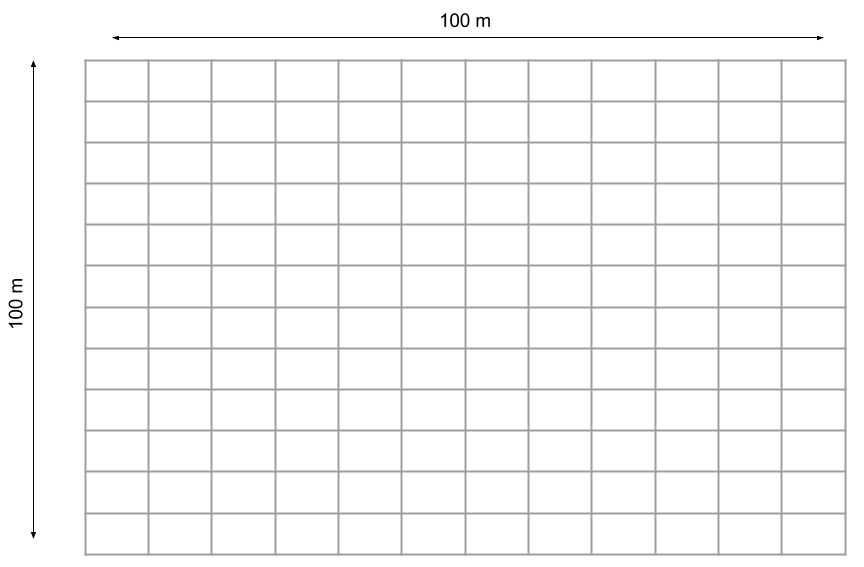
\includegraphics[width=\textwidth/2]{simulation_grid.png}
	\caption{ Gridded simulation area.}	
	\label{fig:simulation_grid}
\end{figure}

The size of individual cells can be configured to increase/decrease the resolution and, therefore, the accuracy of the simulation. As the simulation progresses, plant's grow, their spatial coverage increases, and they enter new grid cells. When a plant enters a new grid cell, it becomes a member of it and cell resources must be distributed to it as well as all other plants present in the given cell. The information associated to each individual grid cell can be split into two categories: \textit{time-dependent} and \textit{simulation-dependent}. The time-dependent information depends only on the current month, is identical for every grid cell and is comprised of: the \textit{soil humidity} and the \textit{illumination}. The simulation-dependent information changes throughout the simulation as plants spawn, die and grow and is comprised of: the list of plants whose roots intersect the cell and the list of plants whose canopy intersects the cell.

\subsection{Resource Distribution}

The strength of each plant in the simulation must be recalculated on a monthly basis. To determine the strength of a given plant, it is necessary to know the illumination and humidity allocated to it along with the temperature. The temperature is not a distributable resource and is identical for all plant instance for a given month. The allocated humidity and illumination is determined by averaging the resources distributed to it in each cell it overlaps in the grid. So, before the strengths of individual plant instances can be calculated, first each cell of the grid must be iterated over and illumination and humidity distributed to the plants contained within. How these are allocated is discussed below.

\subsubsection{Illumination Distribution}

Plants which are heavily dependent on illumination will often grow a large canopy in order to maximize the leaf coverage area which receives direct sunlight. In the process this will restrict the illumination received by smaller plants in the undergrowth. To model the shade projection of larger plants illumination is distributed in each cell depending on the plants height and canopy width. 

Equation \ref{eq:illum_distribution} is used to allocation illumination amongst the set \textit{S} = {P$_{1}$, P$_{2}$, P$_{3}$, ...} of plants which canopy intersect with cell \textit{C$_{xy}$}.

\begin{equation}
\centering
Illumination(P_{n}) = 
\begin{cases}
	C_{illumination}, & \text{if } CanopyWidth(P_{n}) = 0 for x \in S \\
	C_{illumination}, & \text{if } Height(P_{n}) > height(x) for x \in S : x \neq P_{n} \\
    0,              & \text{otherwise}
\end{cases}
\label{eq:illum_distribution}
\end{equation}
Where:
\begin{itemize}
\item \textit{Illumination($P_{n}$)} is the illumination allocated to plant \textit{P$_{n}$}.
\item \textit{C$_{illumination}$} is the monthly illumination of the cell.
\item \textit{CanopyWidth(P$_{n}$)} is the canopy width of plant P$_{n}$.
\item \textit{Height(P$_{n}$)} is the height of plant P$_{n}$.
\end{itemize}

Intuitively, if all plants present in the given cell are canopy-free (i.e no shade projection), the equation allocates them all available illumination. If not all plants are canopy-free, the equation allocated all illumination to the tallest canopy plant leaving all others with zero illumination.


